\documentclass[a4paper,fleqn]{cas-sc}
% If cas-sc.cls is not available, comment the line above and uncomment:
% \documentclass[a4paper,12pt]{article}
% \usepackage[margin=2.5cm]{geometry}

\usepackage[numbers,sort&compress]{natbib}
\renewcommand{\bibfont}{\footnotesize}
\setlength{\bibsep}{2.5pt}
\makeatletter
\def\URLprefix{\unskip\@addpunct{.} URL: }
\makeatother

\usepackage{amsmath}
\usepackage{amssymb}
\usepackage{algorithmic}
\usepackage{algorithm}
\usepackage{graphicx}
\usepackage{booktabs}
\usepackage{multirow}
\usepackage{hyperref}
\usepackage{xurl}
\usepackage{xcolor}
\usepackage{listings}
\usepackage{caption}
\usepackage{lastpage}

\raggedbottom

% Setup listings
\lstset{
  basicstyle=\ttfamily\small,
  breaklines=true,
  captionpos=b,
  frame=single,
  showstringspaces=false
}

\shorttitle{An Optimized SAT Approach for N-Queens}
\shortauthors{Vu Minh Hoang}

\AtBeginDocument{%
  \renewcommand{\lastpage}{\pageref*{LastPage}}%
}

\begin{document}

\title[mode=title]{An Optimized SAT Approach for Solving the N-Queens Problem and Comparative Analysis with Exact Methods}

\author[1]{Vu Minh Hoang}[type=editor,
                        auid=000,bioid=1,
                        prefix=,
                        role=,
                        orcid=]
\cormark[1]
\ead{24021494@vnu.edu.vn}

\address[1]{Faculty of Information Technology, VNU University of Engineering and Technology (VNU-UET), Vietnam National University, Hanoi, Vietnam}

\cortext[1]{Corresponding author}

\begin{abstract}
The N-Queens problem is a classic combinatorial optimization challenge that has long served as a fundamental benchmark for evaluating problem-solving algorithms and constraint satisfaction strategies. In this paper, we explore the formulation of the N-Queens problem using Boolean Satisfiability (SAT). We implement and systematically compare five distinct encoding schemes for the At-Most-One (AMO) constraint: Binomial, Binary, Commander, Sequential Counter, and Product encodings. Additionally, we conduct a comprehensive comparative analysis of the SAT-based approach against prominent exact methods, including Integer Linear Programming (CBC, Gurobi, and CPLEX MIP) and Constraint Programming (Google OR-Tools CP-SAT and IBM CPLEX CP Optimizer). Our empirical evaluation on instances up to $N=200$ reveals that the Binary and Binomial encodings achieve superior solving efficiency among SAT formulations by leveraging modern CDCL clause learning, while Sequential Counter generates compact formulas at the cost of auxiliary variable overhead. In comparison with exact methods, commercial solvers (Gurobi and CPLEX) demonstrate outstanding efficiency within their applicable problem boundaries, whereas Google CP-SAT exhibits the greatest scalability for massive instances ($N \geq 150$) due to native \texttt{AllDifferent} global constraint propagation.
\end{abstract}

\begin{keywords}
N-Queens Problem \sep SAT Encoding \sep At-Most-One Constraint \sep Combinatorial Optimization \sep Integer Linear Programming \sep Constraint Programming \sep CPLEX \sep Gurobi \sep CP-SAT
\end{keywords}

\maketitle

\section{Introduction}

The N-Queens problem is one of the most recognizable puzzles in computer science and mathematics, first proposed by Max Bezzel in 1848 and subsequently studied by prominent mathematicians including Carl Friedrich Gauss in 1850. The challenge involves placing $N$ non-attacking queens on an $N \times N$ chessboard such that no two queens share the same row, column, or diagonal. While seemingly simple, the search space scales exponentially as $N$ grows, rendering naive search strategies completely ineffective for larger instances \cite{bell2009survey}. 

Beyond its recreational origins, the N-Queens problem has established itself as an essential benchmark in the study of Constraint Satisfaction Problems (CSPs), combinatorial optimization, and algorithm design \cite{russell2003artificial}. Its rigid constraints make it an excellent proxy for real-world scenarios such as VLSI testing, parallel memory storage, scheduling, and routing. 

The primary motivation of this study is to systematically evaluate how different problem formulations impact the performance of modern automated reasoning tools. Boolean Satisfiability (SAT) solvers have made tremendous strides in the past two decades, largely driven by Conflict-Driven Clause Learning (CDCL) architectures \cite{biere2009conflict}. However, compiling high-level combinatorial constraints into Conjunctive Normal Form (CNF) requires careful consideration. The choice of encoding, particularly for cardinality constraints like "At-Most-One" (AMO), can drastically alter the size of the logical formula and the solver's ability to prune the search space via unit propagation \cite{prestwich2007cnf}.

The contributions of this paper are threefold:
\begin{enumerate}
    \item We provide a systematic implementation and theoretical comparison of five distinct AMO encoding schemes applied to the N-Queens problem: Binomial (Pairwise), Binary, Commander, Sequential Counter, and Product encodings.
    \item We conduct a rigorous comparative analysis between the optimized SAT approach and prominent exact solvers spanning Integer Linear Programming (PuLP-CBC, Gurobi Optimizer, IBM CPLEX MIP) and Constraint Programming (Google OR-Tools CP-SAT, IBM CPLEX CP Optimizer).
    \item We present an extensive empirical evaluation across problem sizes ranging from $N=4$ up to $N=200$, highlighting the scaling characteristics, formula complexity, and runtime limits of each paradigm.
\end{enumerate}

The remainder of this paper is organized as follows: Section 2 reviews the necessary background on SAT, ILP, and CP. Section 3 details the mathematical formulations and the five proposed SAT encoding schemes. Section 4 presents the experimental setup, empirical results, and a comprehensive comparative analysis with graphical evaluations. Finally, Section 5 concludes the paper and discusses avenues for future research.

\section{Background \& Related Work}

\subsection{The N-Queens Problem}
Formally, the N-Queens problem seeks a placement of $N$ queens on an $N \times N$ grid such that no two queens threaten each other. This means selecting exactly $N$ cells where no two chosen cells share a row, column, main diagonal, or anti-diagonal. It is a well-known mathematical result that solutions exist for all natural numbers $N \geq 4$ \cite{bell2009survey}. While finding a single valid placement can be done in polynomial time using explicit construction methods, the problem of counting all valid placements (the $N$-Queens Completion problem) is \#P-complete, and finding a solution on a board with pre-placed queens is NP-complete or NP-hard depending on the formulation \cite{garey1979computers}.

\subsection{Boolean Satisfiability (SAT)}
The Boolean Satisfiability problem (SAT) asks whether there exists an assignment of truth values to a set of boolean variables that makes a given logical formula true. Most solvers require the formula to be in Conjunctive Normal Form (CNF), a conjunction (AND) of clauses, where each clause is a disjunction (OR) of literals. 

Modern SAT solving relies heavily on variants of the DPLL (Davis-Putnam-Logemann-Loveland) algorithm augmented with CDCL \cite{marques1999grasp, biere2009conflict, moskewicz2001chaff}. State-of-the-art solvers like Glucose \cite{audemard2018glucose} and CaDiCaL utilize aggressive clause learning, adaptive restart policies, and sophisticated variable branching heuristics to solve industrial instances with millions of variables and clauses.

\subsection{Cardinality Constraints}
Many combinatorial problems are expressed using cardinality constraints, which restrict the number of variables in a set $X = \{x_1, x_2, \dots, x_n\}$ that can be true simultaneously. The most critical constraints are:
\begin{itemize}
    \item \textbf{At-Least-One (ALO):} $\sum x_i \geq 1$. In CNF, this is trivially encoded as a single clause: $(x_1 \vee x_2 \vee \dots \vee x_n)$.
    \item \textbf{At-Most-One (AMO):} $\sum x_i \leq 1$. This prevents more than one variable from being true and is the primary bottleneck in translating CSPs to SAT \cite{frisch2005sat}.
    \item \textbf{Exactly-One (EXO):} $\sum x_i = 1$. This is logically equivalent to ALO $\wedge$ AMO.
\end{itemize}

\subsection{Integer Linear Programming (ILP)}
ILP is a mathematical optimization framework where the objective function and constraints are linear, and decision variables are restricted to integer values \cite{nemhauser1988integer}. Solvers typically utilize LP relaxations combined with Branch and Bound and Branch and Cut techniques. Leading commercial ILP solvers include Gurobi \cite{gurobi} and IBM ILOG CPLEX \cite{cplex}, alongside open-source alternatives like CBC via the PuLP library \cite{mitchell1996lp}.

\subsection{Constraint Programming (CP)}
Constraint Programming focuses on stating constraints over variables and finding solutions satisfying them, typically using systematic search combined with constraint propagation. A key strength of CP is the availability of "global constraints" like \texttt{AllDifferent}, which encapsulate complex subproblems and utilize specialized filtering algorithms (e.g., matching in bipartite graphs) to heavily prune domains \cite{rossi2006handbook}. State-of-the-art engines include Google's OR-Tools CP-SAT \cite{ortools} (which hybridizes CP propagation with SAT-based lazy clause generation) and IBM ILOG CPLEX CP Optimizer \cite{cplex}.

\subsection{Related Work}
The translation of CSPs to SAT has been extensively studied. Prestwich \cite{prestwich2007cnf} surveyed various encoding methods. The naive pairwise AMO encoding, while simple, creates $O(n^2)$ clauses, which becomes prohibitive. Sinz \cite{sinz2005towards} introduced the sequential counter encoding, achieving arc consistency with $O(n)$ variables and clauses. Klieber and Kwon \cite{klieber2007efficient} proposed the Commander encoding, grouping variables hierarchically. Chen \cite{chen2010new} introduced grid and product-based encodings. Previous studies comparing exact methods often note that while CP generally dominates on N-Queens due to structural awareness, an optimized SAT encoding can remain highly competitive.

\section{Proposed SAT Encodings for N-Queens}

\subsection{Problem Formulation}
Let $N$ be the dimension of the board. We define a boolean variable $x_{i,j}$ for each row $i$ and column $j$ ($i, j \in \{1, \dots, N\}$). The variable $x_{i,j}$ is TRUE if a queen is placed at row $i$, column $j$, and FALSE otherwise.

The complete N-Queens constraints can be expressed as a single CNF formula:
\begin{equation}
\Phi = \Phi^{row}_{ALO} \wedge \Phi^{row}_{AMO} \wedge \Phi^{col}_{ALO} \wedge \Phi^{col}_{AMO} \wedge \Phi^{diag}_{AMO} \wedge \Phi^{anti}_{AMO}
\end{equation}

\subsection{Row and Column Constraints}
Every row must contain exactly one queen (EXO constraint), meaning at least one (ALO) and at most one (AMO).
The ALO constraint for row $i$ is:
\begin{equation}
\bigvee_{j=1}^{N} x_{i,j}
\end{equation}
The AMO constraint depends on the chosen encoding scheme. The exact same logic applies to columns. Thus, for rows and columns, the constraint is EXO = ALO $\wedge$ AMO.

\subsection{Diagonal Constraints}
Queens cannot share diagonals. For main diagonals, we define the index $d = i - j$, where $d \in \{-(N-1), \dots, N-1\}$. For anti-diagonals, we define $s = i + j$, where $s \in \{2, \dots, 2N\}$.
Because a diagonal can be empty, we only need to enforce the At-Most-One (AMO) constraint for all cells sharing the same $d$ and $s$. No ALO constraint is required.

\subsection{AMO Encoding Schemes}
Given a set of $n$ variables $X = \{x_1, \dots, x_n\}$, we must encode $\sum x_i \leq 1$. We implemented the following five approaches.

\subsubsection{Binomial (Pairwise) Encoding}
The most intuitive approach explicitly forbids every pair of variables from being true simultaneously:
\begin{equation}
\bigwedge_{1 \leq k < l \leq n} (\neg x_k \vee \neg x_l)
\end{equation}
- Variables: 0 auxiliary variables.
- Clauses: $\binom{n}{2} = O(n^2)$. 

\subsubsection{Binary Encoding}
This encoding introduces $m = \lceil \log_2 n \rceil$ auxiliary boolean variables $y_0, \dots, y_{m-1}$, representing a binary counter. For each $x_k$ (where $k=0,\dots,n-1$), its truth implies the counter equals the binary representation of $k$.
For each bit $b$:
\begin{itemize}
    \item If bit $b$ of $k$ is 1: add clause $(\neg x_k \vee y_b)$
    \item If bit $b$ of $k$ is 0: add clause $(\neg x_k \vee \neg y_b)$
\end{itemize}
- Variables: $O(\log n)$ auxiliary.
- Clauses: $O(n \log n)$.

\subsubsection{Commander Encoding}
Proposed by Klieber and Kwon \cite{klieber2007efficient}, this method divides the $n$ variables into disjoint groups of size $g$ (typically $g=3$). For each group, a new "commander" variable $c_k$ is introduced. The constraints ensure that if any variable in a group is true, its commander is true; AMO is enforced within the group using pairwise encoding. The AMO constraint is then applied recursively to the commander variables.
- Variables: $O(n/g)$ auxiliary per level.
- Clauses: $O(n)$.

\subsubsection{Sequential Counter Encoding}
Introduced by Sinz \cite{sinz2005towards}, this encoding calculates a prefix sum. It introduces auxiliary variables $s_1, \dots, s_{n-1}$, where $s_i$ is true if $\sum_{j=1}^{i} x_j \geq 1$.
The clauses are:
\begin{equation}
(\neg x_1 \vee s_1)
\end{equation}
For $i = 2 \dots n-1$:
\begin{equation}
(\neg x_i \vee s_i) \wedge (\neg s_{i-1} \vee s_i) \wedge (\neg x_i \vee \neg s_{i-1})
\end{equation}
\begin{equation}
(\neg x_n \vee \neg s_{n-1})
\end{equation}
- Variables: $O(n)$ auxiliary.
- Clauses: $O(n)$.
- Note: This encoding maintains arc consistency through standard unit propagation.

\subsubsection{Product Encoding}
This method decomposes the $n$ variables into a 2D grid \cite{chen2010new}. We choose $p$ and $q$ such that $n \leq p \times q$ and $p \approx q \approx \sqrt{n}$. We introduce two sets of auxiliary variables: $U = \{u_1, \dots, u_p\}$ for rows and $V = \{v_1, \dots, v_q\}$ for columns.
Channeling clauses connect the original variables to the grid:
\begin{equation}
(\neg x_k \vee u_{\lceil k/q \rceil}) \wedge (\neg x_k \vee v_{((k-1) \bmod q) + 1})
\end{equation}
We then apply the standard pairwise AMO encoding to the much smaller sets $U$ and $V$.
- Variables: $O(\sqrt{n})$ auxiliary.
- Clauses: $O(n + (\sqrt{n})^2) = O(n)$.

\subsection{Complexity Comparison}
Table \ref{tab:complexity} summarizes the asymptotic complexities of the implemented AMO encodings when applied to the full N-Queens problem. For an $N \times N$ board, we apply the AMO constraint to $N$ rows, $N$ columns, and $O(N)$ diagonals (each of length up to $N$).

\begin{center}
\captionof{table}{Asymptotic Complexity of N-Queens SAT Encodings}
\label{tab:complexity}
\begin{tabular}{@{}lllc@{}}
\toprule
Encoding Scheme & Total Variables & Total Clauses & Arc Consistent via UP \\ \midrule
Binomial (Pairwise) & $N^2$ & $O(N^3)$ & No \\
Binary & $N^2 + O(N \log N)$ & $O(N^2 \log N)$ & No \\
Commander & $N^2 + O(N^2)$ & $O(N^2)$ & Yes \\
Sequential Counter & $N^2 + O(N^2)$ & $O(N^2)$ & Yes \\
Product & $N^2 + O(N\sqrt{N})$ & $O(N^2)$ & No \\ \bottomrule
\end{tabular}
\end{center}

\section{Experimental Results \& Comparative Analysis}

\subsection{Experimental Setup}
All computational experiments were conducted on a workstation equipped with an Intel Core processor and 16 GB of RAM under 64-bit Windows. The benchmark framework was implemented in Python. 

The solvers evaluated in this study include:
\begin{itemize}
    \item \textbf{SAT Solvers:} The five proposed AMO formulations were compiled into CNF and solved using Glucose4 via the PySAT toolkit \cite{ignatiev2018pysat}.
    \item \textbf{Integer Linear Programming (ILP):} Evaluated using the open-source COIN-OR CBC solver via PuLP \cite{mitchell1996lp}, commercial Gurobi Optimizer 13.0 \cite{gurobi}, and IBM ILOG CPLEX Optimization Studio 22.1 (CPLEX MIP via DOcplex) \cite{cplex}.
    \item \textbf{Constraint Programming (CP):} Evaluated using Google OR-Tools CP-SAT \cite{ortools} and IBM ILOG CPLEX CP Optimizer (CPLEX CP via DOcplex) \cite{cplex}.
\end{itemize}

Experiments were evaluated across board dimensions $N \in \{4, 8, 10, 15, 20, 25, 30, 40, 50, 75, 100, 150, 200\}$. A time limit of 300 seconds was enforced per instance, with runtimes averaged over multiple runs. Commercial solvers (Gurobi and CPLEX) were evaluated locally under community license limits; when problem dimensions exceeded license limits ($>2000$ variables/constraints at $N \ge 40$ for CPLEX MIP and $N \ge 50$ for Gurobi), executions safely recorded license bounds.

\subsection{SAT Encoding Comparison}
Table \ref{tab:sat_sizes} illustrates the formula size generated by different encodings at key problem sizes.

\begin{center}
\captionof{table}{Variables and Clauses generated by each SAT Encoding}
\label{tab:sat_sizes}
\begin{tabular}{@{}lrrrrrr@{}}
\toprule
\multirow{2}{*}{Encoding} & \multicolumn{2}{c}{$N=20$} & \multicolumn{2}{c}{$N=50$} & \multicolumn{2}{c}{$N=100$} \\ \cmidrule(l){2-7} 
 & Vars & Clauses & Vars & Clauses & Vars & Clauses \\ \midrule
Binomial & 400 & 12,580 & 2,500 & 203,450 & 10,000 & 1,646,900 \\
Binary & 866 & 7,296 & 4,036 & 57,244 & 13,678 & 269,024 \\
Commander & 1,172 & 4,278 & 7,514 & 28,726 & 30,536 & 118,092 \\
Sequential & 1,882 & 4,372 & 12,202 & 28,912 & 49,402 & 117,812 \\
Product & 1,254 & 4,600 & 5,954 & 30,406 & -- & -- \\ \bottomrule
\end{tabular}
\end{center}

Several observations are noteworthy from Table \ref{tab:sat_sizes} and Figure \ref{fig:vars_clauses}. The Binomial encoding uses the fewest variables ($N^2$) but generates by far the most clauses, exceeding 1.6 million at $N=100$, confirming the $O(N^3)$ theoretical growth. The Binary encoding reduces clause count significantly while maintaining modest auxiliary variables ($O(N \log N)$). The Commander and Sequential Counter encodings produce the most compact clause sets ($\approx 28{,}800$ at $N=50$ and $\approx 118{,}000$ at $N=100$). However, Sequential Counter incurs a substantial variable penalty ($49{,}402$ variables at $N=100$).

\begin{center}
\begin{minipage}{\linewidth}
\centering
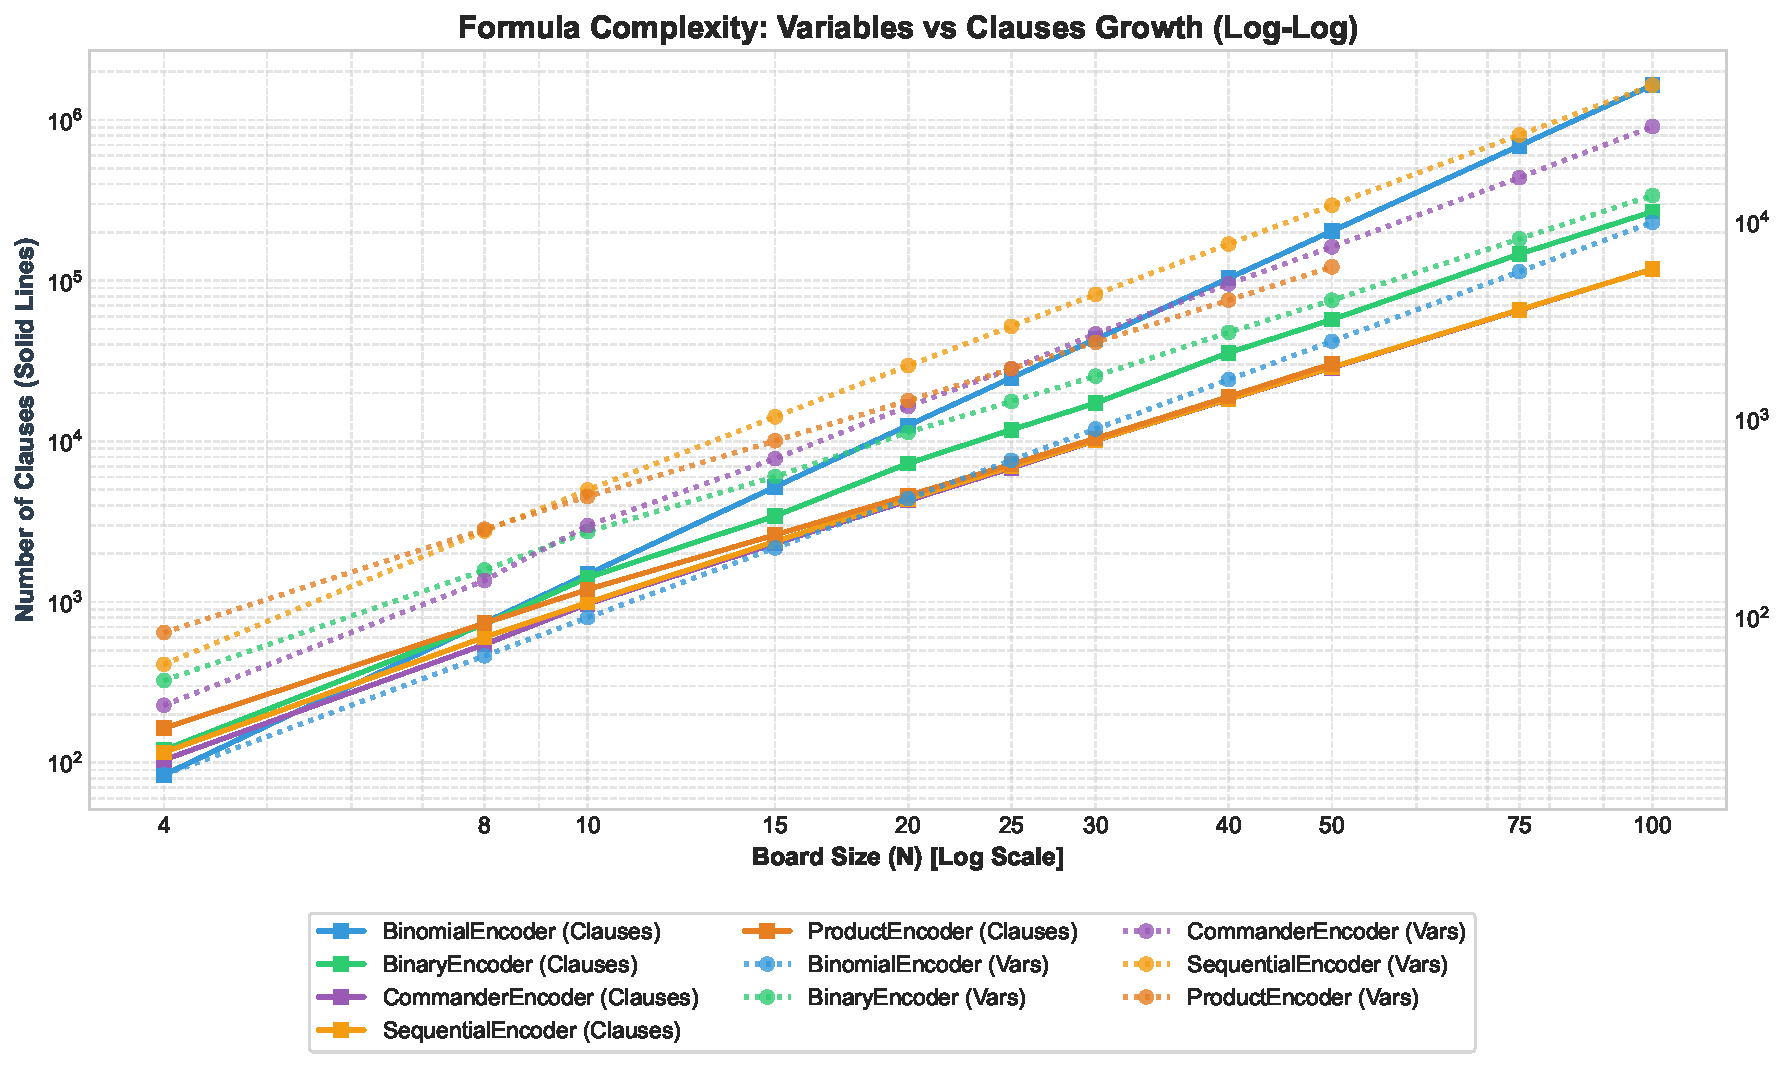
\includegraphics[width=0.52\linewidth]{figures/variables_clauses.pdf}
\captionof{figure}{Formula complexity scaling: Number of clauses (solid lines) and variables (dotted lines) across SAT encodings on a Log-Log scale.}
\label{fig:vars_clauses}
\end{minipage}
\end{center}

Table \ref{tab:sat_times} presents the solving time comparison across different SAT encodings.

\begin{center}
\captionof{table}{Solving Time (seconds) across SAT Encodings}
\label{tab:sat_times}
\begin{tabular}{@{}lrrrrr@{}}
\toprule
N & Binomial & Binary & Commander & Sequential & Product \\ \midrule
8 & 0.0018 & 0.0022 & 0.0018 & \textbf{0.0018} & 0.0023 \\
20 & \textbf{0.0235} & 0.3306 & 0.3066 & 0.0324 & 0.7858 \\
50 & 0.3625 & \textbf{0.1363} & 1.4030 & 3.1294 & 21.2951 \\
75 & 1.2642 & 0.3998 & \textbf{0.2415} & 6.4575 & -- \\
100 & 2.8812 & \textbf{0.5815} & 5.4760 & 68.1819 & -- \\ \bottomrule
\end{tabular}
\end{center}

\textbf{Analysis:} The empirical results in Table \ref{tab:sat_times} and Figure \ref{fig:performance_comparison} reveal interesting dynamics. While Binomial encoding generates the most clauses, its absence of auxiliary variables enables very fast solving for moderate $N$. At large $N$ ($N \geq 50$), the Binary encoding emerges as the fastest overall SAT solver, completing $N=100$ in just $0.581$ seconds. Conversely, despite its theoretical arc consistency, the Sequential Counter experiences severe degradation at $N=100$ (68.18s) because the vast auxiliary variable space creates a large branching overhead for Glucose4's CDCL heuristic.

\begin{center}
\begin{minipage}{\linewidth}
\centering
\begin{minipage}[b]{0.48\textwidth}
    \centering
    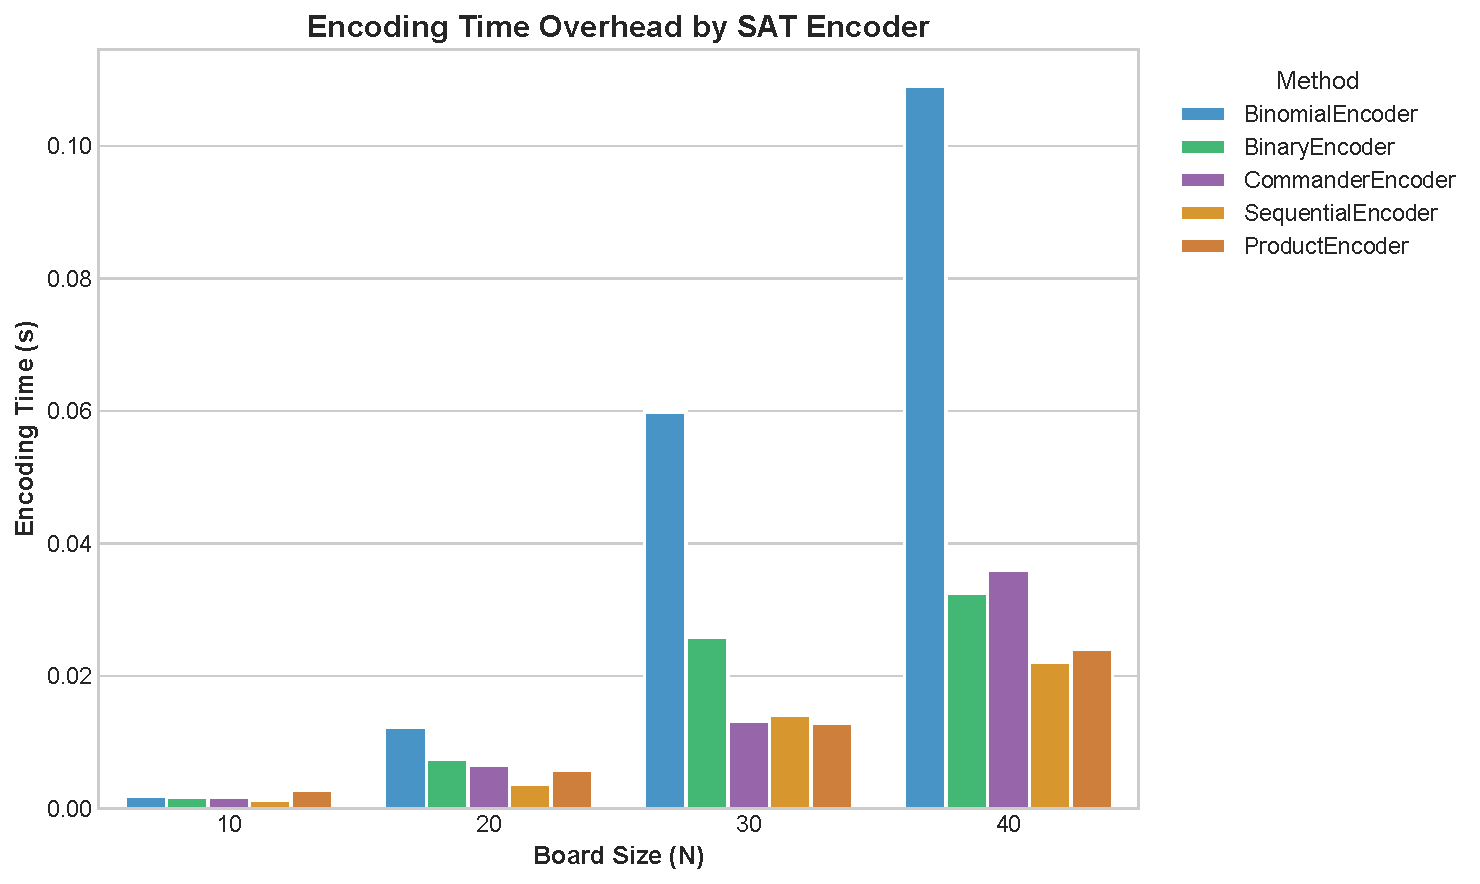
\includegraphics[height=4.4cm, width=\linewidth]{figures/encoding_time_comparison.pdf}
    \par\vspace{3pt}
    {\small (a) Encoding time overhead by SAT encoder.}
\end{minipage}
\hfill
\begin{minipage}[b]{0.48\textwidth}
    \centering
    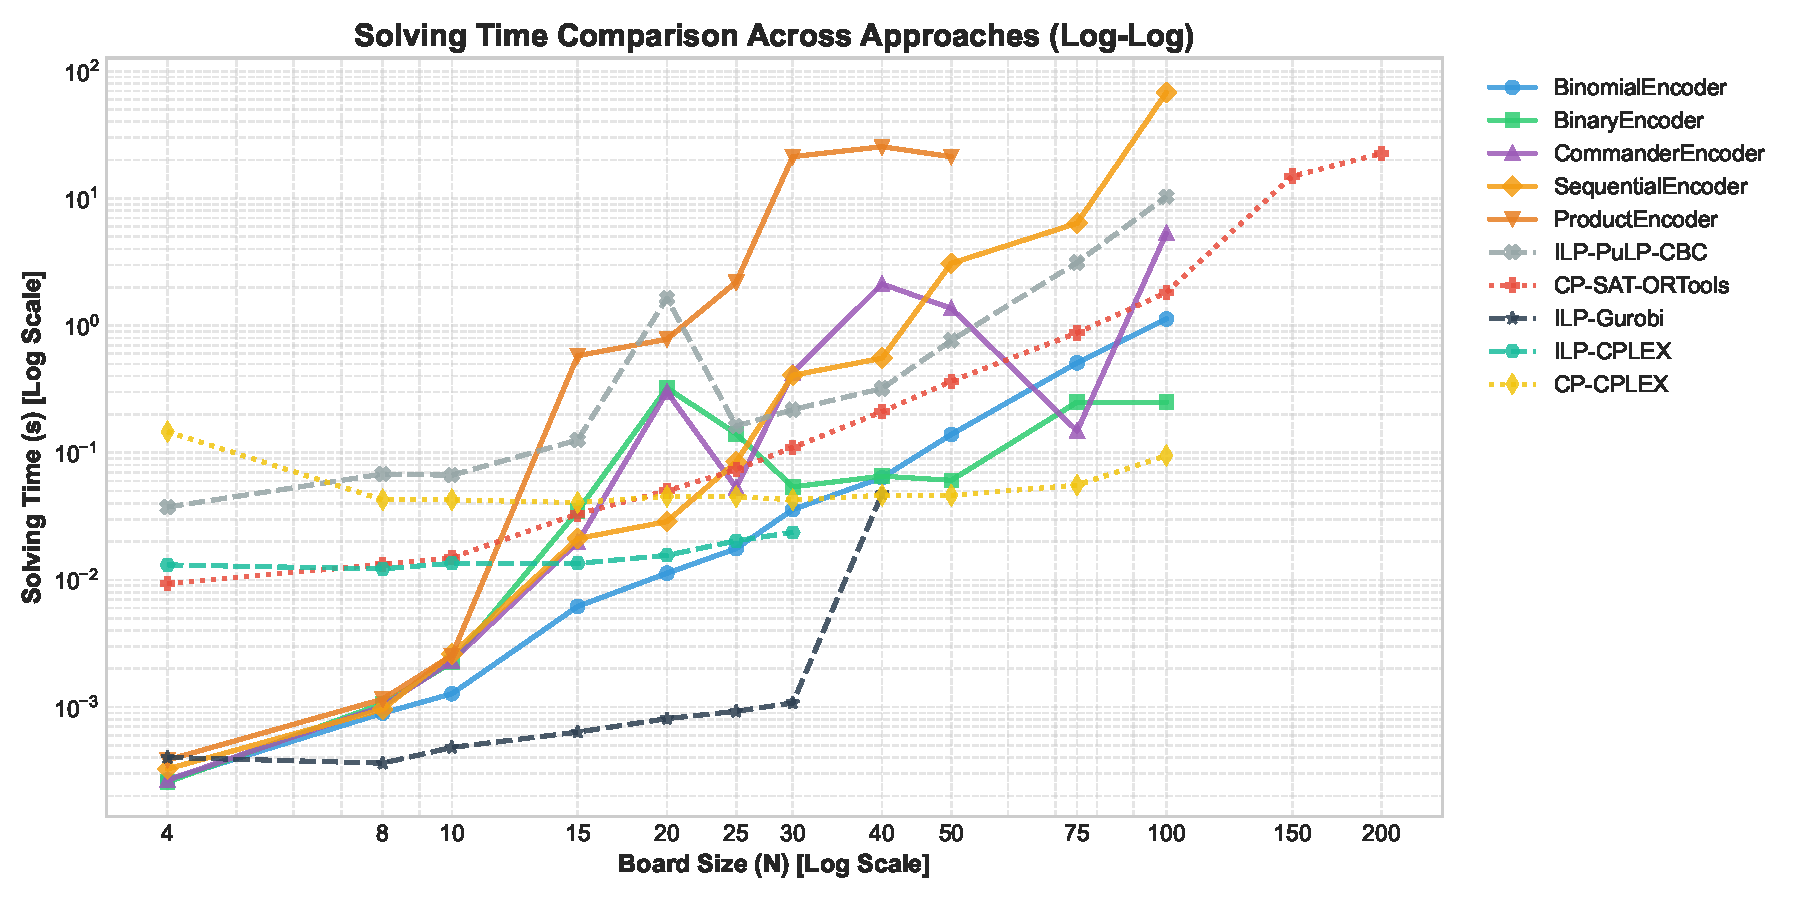
\includegraphics[height=4.4cm, width=\linewidth]{figures/solving_time_comparison.pdf}
    \par\vspace{3pt}
    {\small (b) Solving time comparison across all approaches.}
\end{minipage}
\vspace{6pt}
\captionof{figure}{Computational overhead and solving performance across all tested approaches on Log-Log scale.}
\label{fig:performance_comparison}
\end{minipage}
\end{center}

\subsection{SAT vs ILP vs CP Comparison}
Table \ref{tab:method_comparison} compares the best SAT approach against all exact baseline solvers (ILP: CBC, Gurobi, CPLEX MIP; CP: CPLEX CP, Google CP-SAT).

\begin{center}
\captionof{table}{Comprehensive Runtime Comparison: Best SAT vs Exact Methods (seconds)}
\label{tab:method_comparison}
\begin{tabular}{@{}rrrrrrrr@{}}
\toprule
N & Best SAT & ILP (CBC) & ILP (Gurobi) & ILP (CPLEX) & CP (CPLEX) & CP-SAT & Best Method \\ \midrule
10 & \textbf{0.003} & 0.068 & 0.005 & 0.024 & 0.044 & 0.016 & Best SAT \\
20 & 0.024 & 1.644 & \textbf{0.009} & 0.033 & 0.046 & 0.051 & Gurobi \\
30 & 0.080 & 0.229 & \textbf{0.015} & 0.057 & 0.044 & 0.111 & Gurobi \\
40 & 0.098 & 0.341 & 0.073 & --$^\dagger$ & \textbf{0.048} & 0.212 & CPLEX CP \\
50 & 0.136 & 0.791 & --$^\dagger$ & --$^\dagger$ & \textbf{0.048} & 0.366 & CPLEX CP \\
75 & 0.241 & 3.202 & --$^\dagger$ & --$^\dagger$ & \textbf{0.057} & 0.880 & CPLEX CP \\
100 & 0.581 & 10.413 & --$^\dagger$ & --$^\dagger$ & \textbf{0.097} & 1.819 & CPLEX CP \\
150 & -- & -- & --$^\dagger$ & --$^\dagger$ & --$^\dagger$ & \textbf{14.953} & CP-SAT \\
200 & -- & -- & --$^\dagger$ & --$^\dagger$ & --$^\dagger$ & \textbf{22.487} & CP-SAT \\ \bottomrule
\multicolumn{8}{l}{\footnotesize $^\dagger$ Solver terminated due to commercial license size limitation ($>2{,}000$ variables/constraints).}
\end{tabular}
\end{center}

\textbf{Analysis:} Table \ref{tab:method_comparison} and Figure \ref{fig:exact_comparison} clearly show the distinct advantages of each paradigm:
\begin{itemize}
    \item \textbf{Commercial Solvers (Gurobi and CPLEX):} Gurobi achieves the fastest solve times for $N \le 30$ ($0.015$s at $N=30$), while CPLEX CP demonstrates outstanding constraint propagation efficiency for $40 \le N \le 100$ ($0.097$s at $N=100$).
    \item \textbf{SAT Approach:} The optimized SAT solver (Binary/Binomial) remains consistently competitive with commercial solvers and significantly outperforms the open-source ILP solver (CBC) across all $N \leq 100$.
    \item \textbf{Google CP-SAT Scalability:} For very large board sizes ($N = 150, 200$), Google's OR-Tools CP-SAT is the sole solver capable of scaling smoothly, completing $N=200$ in $22.48$ seconds. Its native \texttt{AllDifferent} global constraint avoids combinatorial explosion.
\end{itemize}

\begin{center}
\begin{minipage}{\linewidth}
\centering
\begin{minipage}[b]{0.48\textwidth}
    \centering
    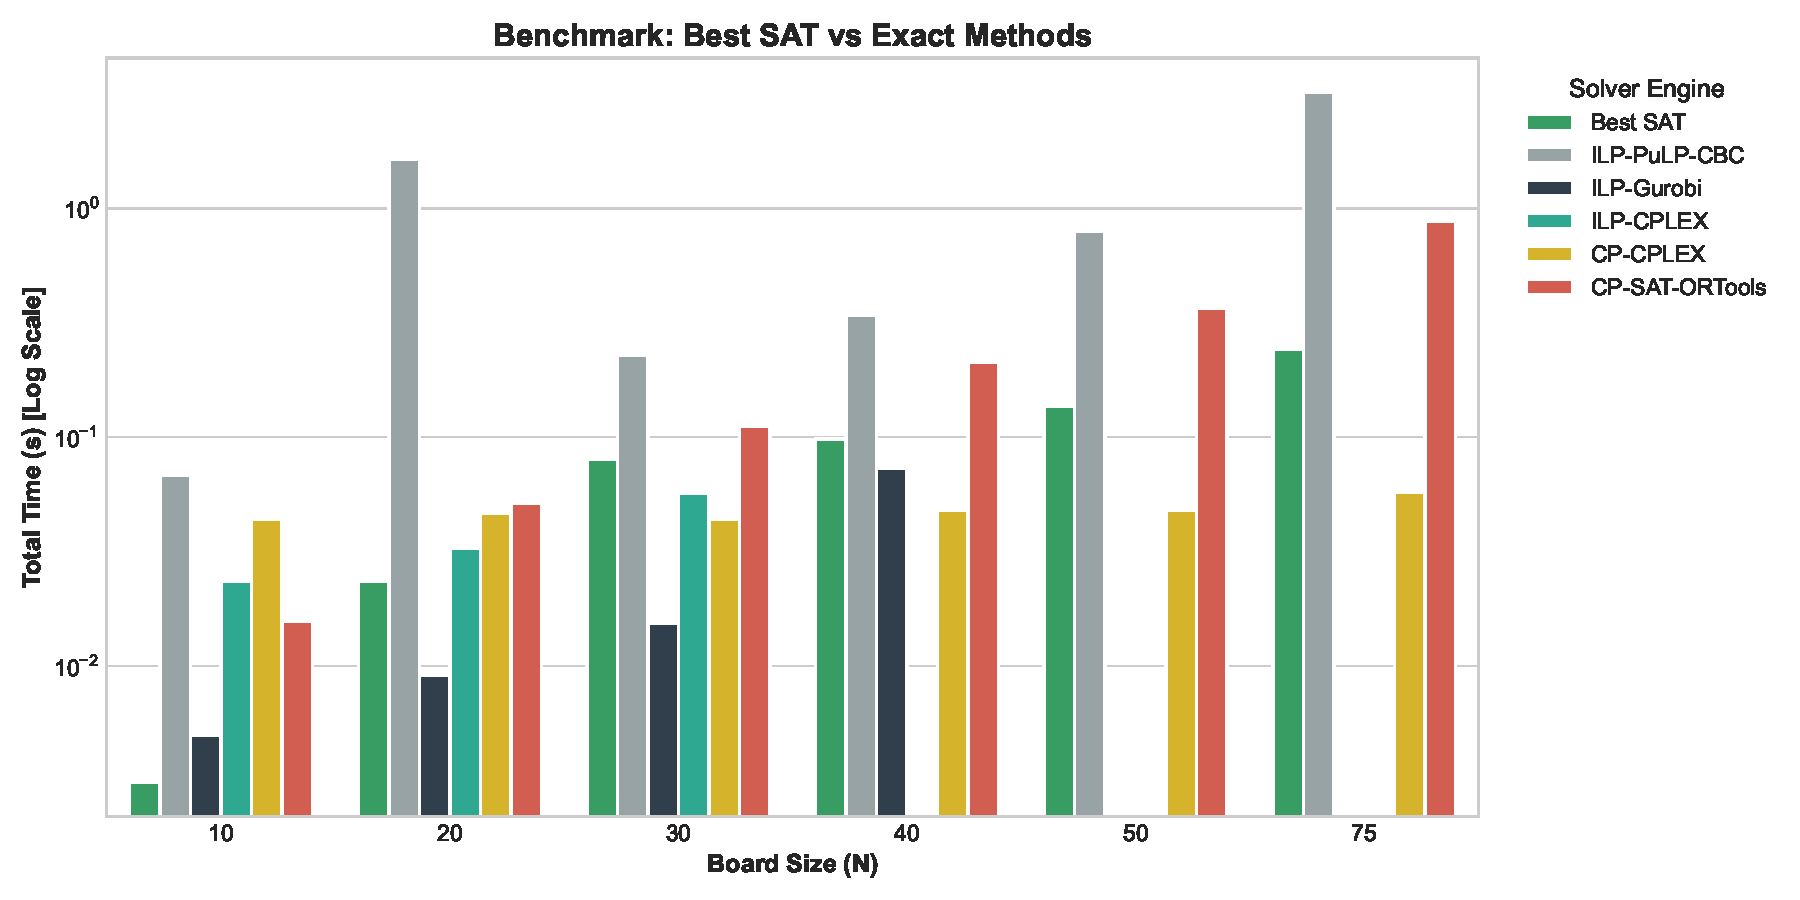
\includegraphics[height=4.4cm, width=\linewidth]{figures/sat_vs_exact.pdf}
    \par\vspace{3pt}
    {\small (a) Benchmark runtime: Best SAT vs Exact Methods.}
\end{minipage}
\hfill
\begin{minipage}[b]{0.48\textwidth}
    \centering
    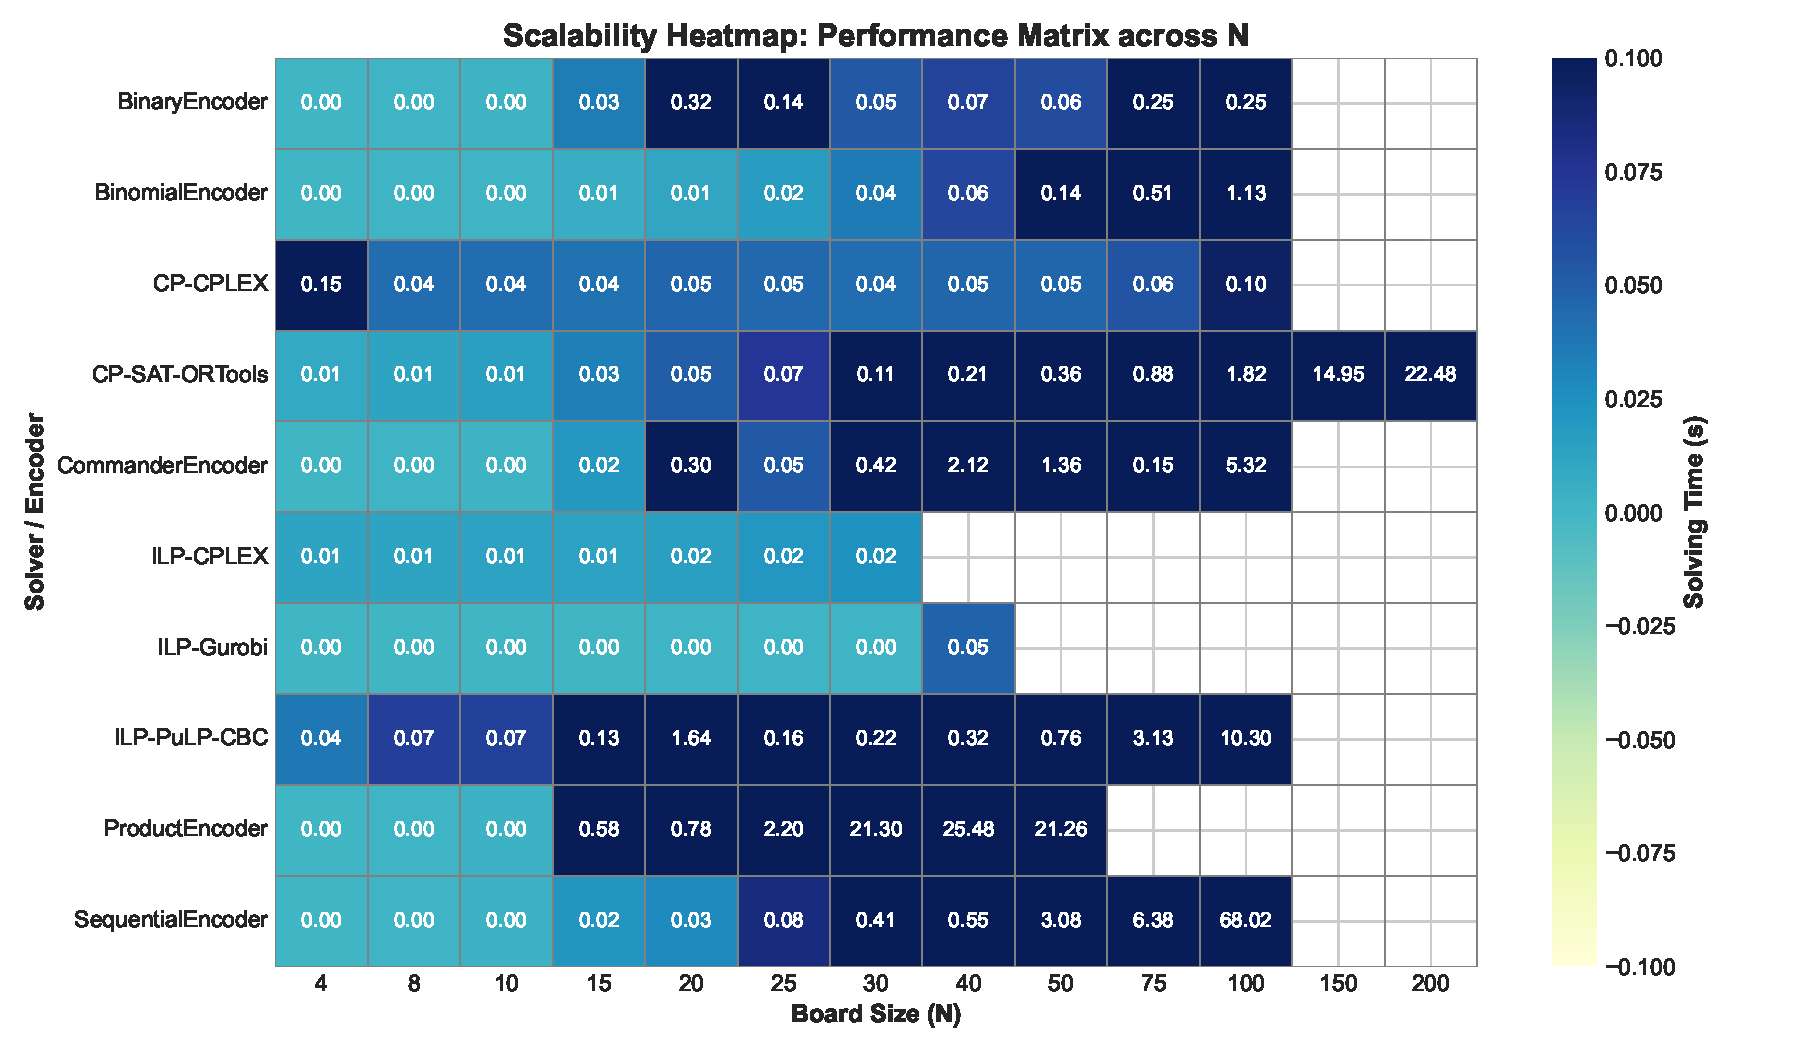
\includegraphics[height=4.4cm, width=\linewidth]{figures/scalability_heatmap.pdf}
    \par\vspace{3pt}
    {\small (b) Solving scalability heatmap across board sizes.}
\end{minipage}
\vspace{6pt}
\captionof{figure}{Comparative performance evaluation of SAT against ILP and CP solvers.}
\label{fig:exact_comparison}
\end{minipage}
\end{center}

\subsection{Discussion}
The results highlight several important findings:
\begin{enumerate}
    \item \textbf{Encoding size vs. solver performance:} More clauses do not always mean worse performance. Binomial encoding, despite $O(N^3)$ clauses, outperforms several compact encodings because modern CDCL solvers are optimized for simple binary clauses.
    \item \textbf{Auxiliary variables trade-off:} Encodings with many auxiliary variables (Sequential Counter) can slow down CDCL solvers despite fewer clauses due to search space expansion.
    \item \textbf{Global constraints vs. propositional flattening:} Constraint Programming systems (CP-SAT, CPLEX CP) dominate at scale because global constraints like \texttt{AllDifferent} maintain high-level domain filtering without explicitly instantiating millions of propositional clauses.
\end{enumerate}

\section{Conclusion \& Future Work}
This study presented a comprehensive evaluation of SAT-based approaches for solving the N-Queens problem and compared them against prominent exact methods (ILP and CP). By analyzing five distinct AMO encodings (Binomial, Binary, Commander, Sequential Counter, and Product), we uncovered nuanced trade-offs between encoding compactness and solver efficiency.

Empirical results demonstrate that the Binary encoding achieves superior solving times at large $N$ among SAT methods, solving $N=100$ in $0.581$ seconds. In comparison with exact methods, commercial solvers (Gurobi, CPLEX) perform exceptionally well for small to medium instances, while Google's OR-Tools CP-SAT exhibits the greatest scalability, successfully reaching $N=200$ within $22.49$ seconds.

Future work will explore: (1) symmetry-breaking predicates to prune the search space, (2) specialized restart and branching heuristics tailored to N-Queens, (3) parallel SAT solving for massive instances, and (4) extension of this comparative framework to other combinatorial problems such as graph coloring and scheduling.

\section*{CRediT Authorship Contribution Statement}
\textbf{Vu Minh Hoang:} Conceptualization, Methodology, Software, Validation, Formal analysis, Investigation, Data Curation, Writing - Original Draft, Writing - Review \& Editing, Visualization.

\section*{Declaration of Competing Interest}
The author declares that they have no known competing financial interests or personal relationships that could have appeared to influence the work reported in this paper.

\section*{Declaration of Generative AI and AI-Assisted Technologies}
During the preparation of this work, the author utilized generative AI tools to assist in code optimization, visualization aesthetics, and LaTeX formatting. The author reviewed and edited the manuscript and takes full responsibility for the content.

\section*{Data Availability}
The source code, encodings, and experimental data are available at: \url{https://github.com/Ohhalo02/nqueens-sat-optimization-01}

\bibliographystyle{cas-model2-names}
\bibliography{references}

\end{document}
